\documentclass[12pt,a4paper]{article}

\usepackage{amsmath}
\usepackage{amssymb}
\usepackage[francais, english]{babel}
\usepackage{color}
\usepackage{eurosym}
\usepackage{fancyhdr}
\usepackage[T1]{fontenc}
\usepackage[bottom=39mm]{geometry}
\usepackage{graphicx}
\usepackage{hyperref}
\usepackage[utf8]{inputenc}
\usepackage{libertine}
\usepackage{listings}
\usepackage{subcaption}
\usepackage{url}
\usepackage{xpatch}

\begin{document}
\newcommand{\HRule}{\rule{\linewidth}{0.5mm}}

\begin{titlepage}
   \begin{sffamily}
      \begin{center}

         
\includegraphics{./images/uvsq_logo.png}\\
         \textsc{\LARGE Université de Versailles Saint-Quentin-en-Yvelines (UVSQ)}\\[2cm]
         \textsc{\Large Rapport de Stage Master 2}\\[1.5cm]

         % Title
         \HRule \\[0.4cm]
         {\huge \bfseries Prototypage d'un module de spécialisation OpenCL\\[0.4cm]}

         \HRule \\[1cm]
         
\includegraphics[width=75mm]{./images/asplus_eolen_logo.png}\\[1cm]

         % Author and supervisor
         \begin{minipage}{0.4\textwidth}
            \begin{flushleft}
               \large \emph{Auteur :} Yanis \textsc{KHORSI}\\
            \end{flushleft}
         \end{minipage}
         \begin{minipage}{0.5\textwidth}
            \begin{flushright}
               \large \emph{Tuteur :} Sébastien \textsc{MONOT}\\
            \end{flushright}
         \end{minipage}

         \vfill

         % Bottom of the page
         {\large 14 Mars 2016 — 16 Septembre 2016}

      \end{center}
   \end{sffamily}
\end{titlepage}


\newpage
\pagestyle{fancy}
\lhead{}
\rhead{Yanis \bsc{KHORSI}}
\cfoot{}
\null
\newpage
\lhead{\rightmark}
\cfoot{\thepage}

\part*{Remerciements}
\sloppy
Je tient à profiter par le biais de ce rapport de stage de fin d'étude, pour
exprimer mes vifs remerciements à toute l'équipe AS+ d'EOLEN, plus
particulièrement ceux qui m'ont encadré tout au long de cette période, notre
chef de projet Sébastien \textsc{Monot}, et nos deux experts techniques Kevin
\textsc{Juilly} et Vincent \textsc{Ducrot}, pour leur accueil chaleureux, leur
patience et leur apprentissage.
\\
\\
Ainsi que tous ceux qui ont contribué de près ou de loin à la réussite de mon
stage, et à ma famille qui m'a toujours soutenu et encouragé à persévérer.
\\
\\
Un merci bien particulier à Kevin \textsc{Juilly}, pour m'avoir prodigué la
passion des Rubik's Cube, en me faisant découvrir de nouvelles techniques de
résolution me rendant plus rapide, on pourra ainsi dire qu'il aura appliqué une
passe d'optimisation sur moi.
\\
\\
Merci à \emph{Bull Atos technologies} d'avoir mis à notre disposition des tables
de ping-pong, nous permettant ainsi de partager quelques moments de détente avec
d'autres membres de Ter@tec, surtout avec notre cher collègue Yohan \textsc{Lee
Tin Yien}.
\\
\\
À Tony \textsc{Delforges} pour la chasse aux Pokémons pendant la pause déjeuner.
\\
\\
Et surtout un grand merci, à mon collègue et ami Stéphane \textsc{Bouhrour}, qui
m'accompagne sur le trajet quotidien vers le bureau le matin, et du retour le
soir pour échanger notamment sur le stage et de nos bogues respectifs, et de
notre enthousiasme autour de musiques et saga audio en tout genre.
\\
\\
Enfin, je remercie toute l'équipe pédagogique du master CHPS de l'UVSQ pour leur
enseignement et initiation au domaine du HPC.

\newpage
\renewcommand{\abstractname}{Résumé}
\begin{abstract}
\end{abstract}
Dans le cadre du calcul Haute Performance (HPC), l'utilisation des accélérateurs
(GPUs ou Xeon Phi) à tendance à augmenter. Malheureusement, très peu de codes
de calcul sont capables d'exploiter toutes les performances de ces matériels.
Les coûts de translation et optimisations appropriées deviennent plus gros, et
les modèles de programmations ne sont pas unifiés, à part quelques initiatives
comme OpenCL. Les technologies actuelles nécessitent généralement un compromis
entre la généricité et la performance. Pourtant, il est clair que les structures
algorithmiques nécessaires pour la plupart des accélérateurs sont similaires et
que cette abstraction suffisante pourrait adresser les différentes
architectures. AS+ en partenariat avec le CEA et l'INRA ont développé dans le
cadre du projet ITEA Mach une chaîne de compilation basée sur le langage R pour
des machines hétérogènes mixant CPUs, GPUs et Xoen Phi. Le backend de cette
chaîne développé par AS+, repose sur une couche d'abstraction, et de modules de
spécialisations pour différentes cibles. Le code optimisé exprimé avec cette
couche d'abstraction ne nécessite pas de réécriture de code, le module de
spécialisation génère automatiquement un code performant pour le matériel ciblé.
Le code exécuté est vue comme un ensemble de tâches avec des dépendances de
données implicites. Le but de mon stage est de mettre en \oe{}uvre l'un des
modules de spécialisation, qui permet de généré du code optimisé en OpenCL.

\renewcommand{\abstractname}{Abstract}
\begin{abstract}
\end{abstract}
In the field of high performance computing (HPC), the use of accelerators (GPUs
or Xeon Phi) is now a strong growth trend. Unfortunately few codes are able to
fully exploit the power of these. The costs of translation and related
optimizations are becoming higher and programming models are not unified,
despite some initiatives like OpenCL. Current technologies typically require a
trade-off betweem genericity and performance. Yet it is clear that algorithmic
structures required for most accelerators are similar and that sufficient
abstraction would address the different architectures. Whitin ITEA MACH project
AS+ teams have jointly developed with CEA and INRA a toolchain for compiling R
language to heterogeneous platforms mixing CPUs, GPUs and Xeon Phi. The backend
of this toolchain, developpend by AS+, relies on an abstraction layer, and
specialization modules for different targets. Optimized code expressed with this
abstraction layer no longer require rewriting and specialization module
automatically generates an efficient code for the target architecture. The code
to be executed can be seen as a set of smaller tasks with implicit data
dependencies. The purpose of my internship is to implement one of the
specialization modules, allowing generated optimized code with OpenCL.


\let\englishtableofcontents\tableofcontents
\patchcmd\englishtableofcontents{{toc}}{{tec}}{}{}
\preto\englishtableofcontents{\begin{otherlanguage}{english}}
\appto\englishtableofcontents{\end{otherlanguage}}
\newcommand{\addetoc}[2]{
   \addcontentsline{tec}{#1}{\protect\numberline{\csname the#1\endcsname}#2}}

\renewcommand{\contentsname}{Sommaire}
\newpage
\tableofcontents{}
\newpage
\englishtableofcontents{}
\newpage
\listoffigures

\newpage
\section{Introduction}
\addetoc{section}{Introduction}
\paragraph{}
On m'a attribué dans le cadre de ce stage que j'ai effectué au sein
d'\emph{AS+}, une filiale du groupe \emph{EOLEN}, la mission de développement
d'un module de spécialisation \emph{OpenCL} en utilisant l'infrastructure de
compilation \emph{LLVM} devant s'intégrer à une chaîne de compilation et
d’exécution pour des architectures hétérogènes et s’appuyant sur les DSL (Domain
Specific Language ou \emph{langages dédiés} en français) mis en place.

Ce travail est inscrit dans le cadre du projet \emph{ITEA Mach}. C'est un projet
européen regroupant une vingtaine de partenaires, dont le \emph{CEA LIST} et
l'\emph{INRA} deux entreprises avec qui travaille plus particulièrement
\emph{AS+} dans le domaine des biostatistiques avec le langage R comme DSL.

\paragraph{}
J’ai intégré l’équipe projet \emph{AS+}, constituée d’un ingénieur d’études
senior -- Gaétan \textsc{Bayle des Courchamps} -- responsable du développement de
l’interface avec le runtime tâche, de deux experts HPC -- Vincent \textsc{Ducrot}
et Kevin \textsc{Juilly} -- en charge des spécifications et de la conception de
la chaîne de compilation et d’exécution, et d’un chef de projet -- Sébastien
\textsc{Monot} -- responsable technique de l’activité HPC et du pilotage des
projets en particulier.

Le projet est en phase finale de développement, j'ai par conséquent basé mon
travail sur un modèle et une architecture logicielle déjà définit, pour
l'intégrer au plus simple au reste de la chaîne.

\paragraph{}
Dans les sections suivantes, je commence par présenter plus en détail
l'entreprise d'accueil et le service auquel je suis affecté, suivra la
présentation du projet \emph{Mach} sur lequel je travail et les logiciels
utilisés comme fondation à son développement. Je poursuivrai avec le déroulement
du travail que j'ai effectué tout au long de ma période de stage, la prise en
main des outils au développement du prototype de spécialisateur et d’autres
éléments de la chaine de compilation. Je montrerai ensuite les résultats obtenus
par ce que j’ai réalisé. Je finirai par une conclusion résumant le travail
effectué et les perspectives attendu de ce projet.

\section{Présentation de l'entreprise et du service}
\addetoc{section}{Company and service presentation}
\paragraph{AS+}
est une société de conseil et d'ingénierie filiale du groupe \emph{EOLEN} depuis
2012. Ce dernier est présent dans différents secteurs tels que les
télécommunications, la finance, l'aéronautique, le spatial, la défense,
l'énergie et les sciences de la vie. Le groupe est principalement implanté en
\emph{Ile-de-France} mais compte aussi une implantation d'une cinquantaine de
personnes au \emph{Brésil}. Le groupe a réalisé plus de 23M\euro{} de chiffre
d'affaire en 2015 et compte environ 300 personnes.

\paragraph{}
AS+ est spécialisé dans les métiers des télécommunications, l'informatique
scientifique et industriel et dans le calcul intensif (HPC).

\paragraph{}
Le bureau d’étude HPC, fort d'une vingtaine de collaborateurs, a développé
depuis plusieurs années une forte expertise sur les méthodes et outils de
développement dédiés aux plates-formes de calcul intensif : architectures
multic\oe{}urs, accélérateurs de type GPU et many-core (Xoen-Phi), clusters de
calcul et a bâti une offre de services complète portant sur le développement,
l’optimisation et le portage sur architectures parallèles de codes de calcul et
suivant des modes d’intervention au plus proche des besoins des clients :
conseil/audit, formations, assistance technique ou prestations clé en main. AS+
compte parmi ses clients les principaux acteurs du domaine en France comme le
\emph{CEA}, \emph{TOTAL}, l’\emph{ONERA}, l’\emph{IDRIS}, l’\emph{ANDRA},
l’\emph{IRSN}, \emph{ATOS/Bull}, \emph{IBM}, \emph{DAHER}.

\paragraph{}
\sloppy
L’équipe HPC intervient également très en amont dans l’écosystème du calcul
intensif aux côtés de partenaires industriels et académiques tels que
l’\emph{INRA}, le \emph{CEA}, \emph{THALES} et ce dans le cadre de projets R\&D
tels que \emph{OpenGPU (FUI)}, \emph{Brainomics (FSN)} \emph{M2DC (H2020)} ou
\emph{MACH (ITEA)}. \emph{AS+} propose également un catalogue de formations
spécifiques au calcul intensif qui comprend notamment des modules dédiés aux
technologies \emph{CUDA}, \emph{OpenCL}, \emph{MPI/OpenMP} ou aux suites
\emph{Intel Parallel Studio / Cluster Studio}.

\paragraph{}
\emph{AS+} est par ailleurs membre de l’association \emph{Ter@tec} depuis 2012
qui rassemble les principaux acteurs académiques et industriels du calcul
intensif en France. La société a, depuis, concrétisé un certain nombre d’actions
en lien direct avec l’association, notamment en participant depuis cinq ans au
forum TERATEC, et la mise en place d'une démarche de partenariats avec d’autres
membres de l’association, tels que \emph{Activeeon}, \emph{Caps Entreprises},
\emph{Nvidia} et \emph{Intel}. De plus la société est installée depuis octobre
2012 sur le Campus \emph{Ter@tec} à Bruyères le Châtel. Cela permet de renforcer
la synergie entre l'équipe R\&D et celle déjà présente au \emph{CEA} et au
\emph{TGCC} (Très Grand Centre de Calcul) qui a la responsabilité du support
applicatif aux utilisateurs du centre de calcul.

\section{Présentation du sujet de stage}
\addetoc{section}{Presentation of the internship}
\subsection{Descriptif général du projet Mach}
\addetoc{subsection}{General description of the Mach project}
\paragraph{ITEA Mach~\cite{mach}}
est un projet européen regroupant une vingtaine de partenaires dont AS+, le
CEA-LIST, l'INRA, Silkan, Thales Communications and Security... L'objectif de ce
projet est de faciliter la programmation sur machines hybrides combinant CPU et
accélérateurs tels que GPU et Xeon-Phi, en partant d'une approche de type DSL
(Domain Specific Language) embarqué si besoin dans un langage hôte (DSeL). Pour
valider les frameworks mis en place, le projet dispose d’un certain nombre de
cas utilisateurs représentatifs de différents domaines : traitement d’image, du
signal, mécanique des fluides, biostatistiques, etc.

\paragraph{}
Le rôle d'AS+ est de fournir les technologies permettant de construire des
chaînes de compilation modulaires construites autour du compilateur LLVM et un
modèle d’exécution de type tâche pour des architectures hétérogènes en
s’appuyant sur les DSL mis en place pour chaque domaine. La société travaille
plus particulièrement avec l’INRA et le CEA-LIST en langage R dans le domaine
des biostatistiques. L’INRA apporte les applications et le CEA-LIST apporte le
frontend de traduction du langage R vers vers une représentation intermédiaire
dont on a besoin dans notre chaîne de compilation, comme le montre la
figure~\ref{toolchain_fr}.

\begin{figure}[h!]
   \begin{center}
      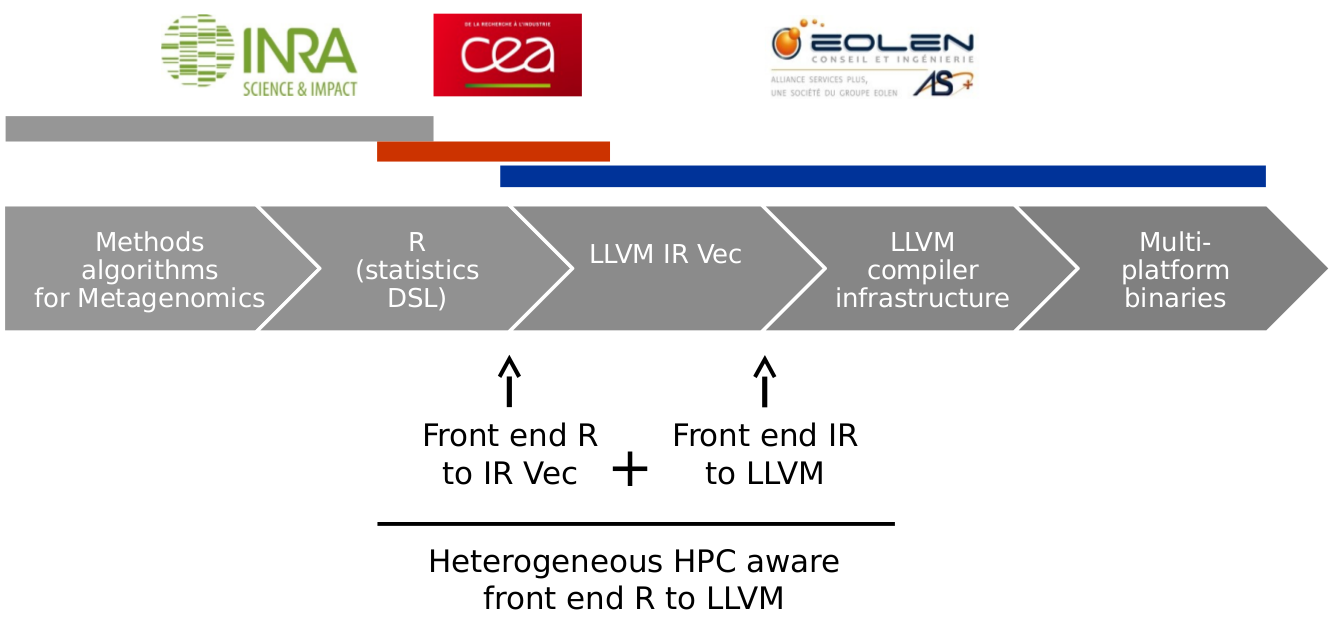
\includegraphics[width=135mm]{./images/toolchain_fr.png}
   \end{center}
   \caption{Chaîne d'outils du partenariat français~\cite{toolchain_fr}}
   \label{toolchain_fr}
\end{figure}

\paragraph{}
On peut décrire la chaîne de compilation développée par AS+ comme ceci : on
prend en entrée du code dans une version étendue du langage LLVM IR, annotée si
besoin pour faciliter la compilation. Le code passe par le tâchifieur
(Parallelizer) qui s'occupe de regrouper en tâches les instructions réalisées et
de les placer dans des procédures. Une fois le programme découpé en tâches, les
codes passent par les différents spécialisateurs pour être transformés en code
LLVM IR pur, avec les annotations adaptées à une architecture spécifique. Ils
peuvent ensuite passer dans la chaîne de compilation standard de LLVM pour être
optimisés et compilés sous forme binaire. La gestion de la mémoire et les appels
aux bibliothèques sont transformés en équivalents fournis par le runtime. Le
tout peut ensuite être regroupé dans un exécutable capable de tourner sur une
machine hétérogène.\\
La figure~\ref{backend_mach} résume tout cela.

\begin{figure}[h!]
   \begin{center}
      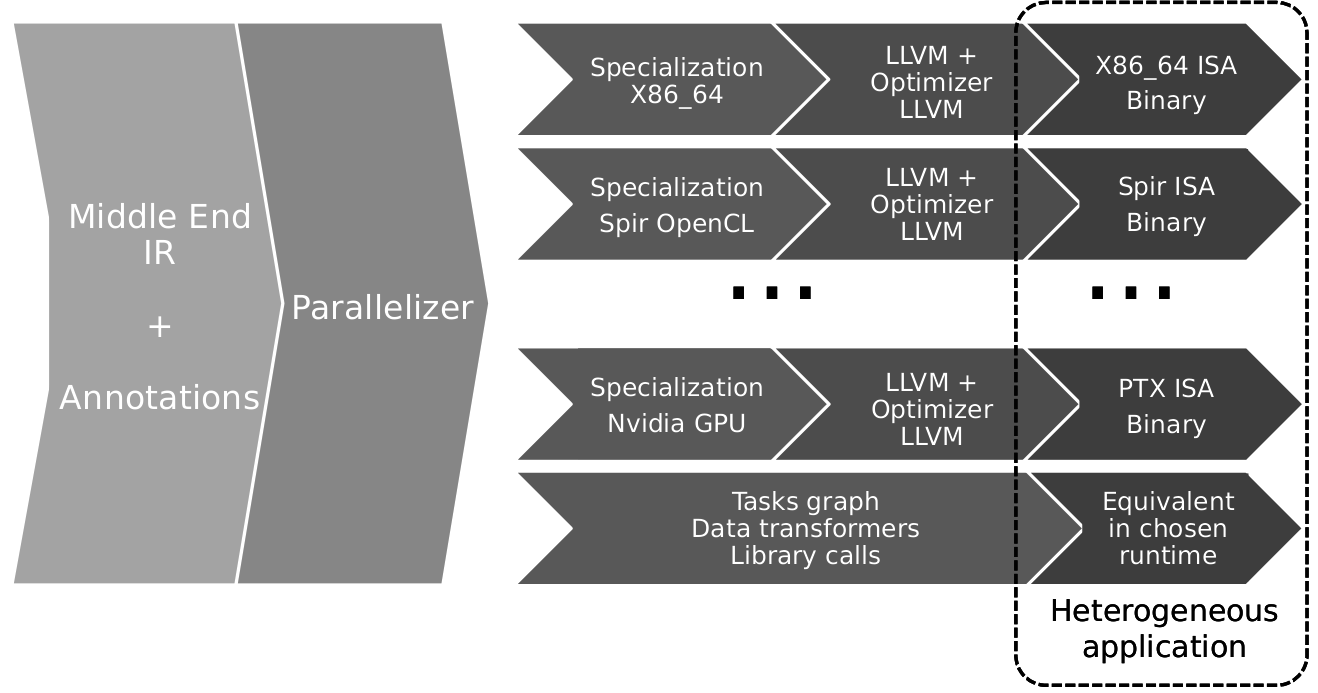
\includegraphics[width=135mm]{./images/backend_mach.png}
   \end{center}
   \caption{Back-end de l'outil de compilation \emph{Mach}~\cite{toolchain_fr}}
   \label{backend_mach}
\end{figure}

\subsection{Runtime}
\addetoc{subsection}{Runtime}
\subsubsection{Mach Runtime}
\addetoc{subsubsection}{Mach Runtime}
\paragraph{}
Nous avons donc besoin d'un runtime hétérogène, qui prendra en charge une
application conçue comme un ensemble de tâches, nous voulons donc lui laisser le
choix de gérer quand et dans quel ordre il va les exécuter, sachant qu'il
connait les accès mémoires de chaque tâche. Il pourra, par conséquent, se
construire un graphe de dépendance de données entre ces dernières, ainsi tout en
respectant un tant soit peu l'ordre dans lequel les tâches lui sont données, le
runtime pouvant les réordonner quand cela permet une exécution parallèle.

Le découpage en tâches de l’application permet une répartition de charge
dynamique sur les différentes ressources de calcul indépendamment de
l’application. Il doit donc être capable de déterminer les unités de calcul
disponibles. Lui incombe également la gestion de la mémoire et la gestion des
allocations et des copies mémoires dans le cas où des unités de calcul accèdent
à de la mémoire différente (comme le CPU et un GPU ou Xeon-Phi).

\paragraph{}
Il existe des runtimes qui répondent à nos attentes, nous allons donc en
utiliser un : StarPU. Mais nous allons tout de même définir une interface
d'abstraction pour limiter l'adhérence au runtime sous-jacent et nous permettre
d'ajouter des fonctionnalités absentes de ce dernier sans avoir à le modifier en
profondeur.

\subsubsection{StarPU}
\addetoc{subsubsection}{StarPU}
\paragraph{}
\sloppy
StarPU est un runtime par tâches pour systèmes multic\oe{}urs hétérogène
développé par l'équipe runtime de l'INRIA de Bordeaux~\cite{starpu}.

\fussy
Il peut gérer les systèmes multi-processeurs, GPU Nvidia en utilisant Cuda et
les différents périphériques répondant à OpenCL (GPU AMD ou Intel Xeon-Phi par
exemple).

Le runtime intègre également un gestionnaire de mémoire. Il est capable de gérer
les dépendances entre les tâches à l’aide des intentions fournies avec ces
tâches. Il fournit également la possibilité de découper les zones mémoires
enregistrées en sous parties, pour pouvoir, par exemple, permettre à des tâches
accédant à des zones différentes de la donnée de tourner en parallèle.

\subsection{LLVM}
\addetoc{subsection}{LLVM}
\subsubsection{Déscription}
\addetoc{subsubsection}{Description}
\paragraph{}
\sloppy
Anciennement appelé \og{} Low Level Virtual Machine \fg{} (Machine Virtuelle de
Bas Niveau en français), \emph{LLVM}~\cite{llvm} est un projet d'infrastructure
de compilation qui permet l'optimisation de code indépendamment de toute
plateforme et de tout langage à différentes étapes de la compilation ou à
l'exécution du programme avec un compilateur à la volée.

Le projet a débuté en 2000 en tant que projet de recherche sous la direction de
Vikram Adve et Chris Lattner à l'Université de l'Illinois à Urbana–Champaign. Il
est à présent distribué sous forme de logiciel libre avec une licence permissive
et il est écrit sous forme de bibliothèques réutilisables.

Il définit une séparation claire des phases de compilation, un langage
intermédiaire et un ensemble de back-ends pouvant générer du code pour une
architecture spécifique.

\paragraph{}
Il propose aussi depuis sa version 2.6 le compilateur Clang pour les langages C,
C++, Objective-C et Objective-C++. Ce front-end se charge de traduire le code en
langage intermédiaire de plus bas niveau, le c\oe{}ur de LLVM applique ensuite
des passes de transformation et d'optimisation de code, et le back-end, le code
en assembleur pour une architecture spécifique.

\paragraph{}
La modularité est un concept clé dans LLVM. Grâce à cette architecture, l'ajout
de la prise en charge d'un nouveau langage de haut niveau se réduit à écrire le
front-end de traduction vers le LLVM IR et la prise en charge d'un nouveau
processeur avec le back-end correspondant. Mais LLVM impose cette séparation des
étapes de manière formelle : le seul outil de communication entre les étapes est
le langage LLVM IR.

\subsubsection{Passes}
\addetoc{subsubsection}{Pass}
\paragraph{}
La partie centrale fonctionne par l'application d’un ensemble de passes. Il y a
deux types de passes dans LLVM : les passes d’analyse, qui génèrent des
statistiques utilisables par d’autres passes sans modification du code ; et les
passes de transformations, qui modifient le code principalement pour l'optimiser
en se basant potentiellement sur les statistiques générées par le premier type
de passe. On peut indiquer des dépendances entre les passes. Celles-ci peuvent
nécessiter le résultat d’une autre passe ou bien invalider le travail d’une
autre, qui sera à exécuter à nouveau.

\subsubsection{IR}
\addetoc{subsubsection}{IR}
\paragraph{}
Le langage intermédiaire utilisé par LLVM est un langage d'assemblage sous forme
SSA (Static Single Assignment), c'est-à-dire qu'on ne peut affecter une valeur à
un registre qu'une seule fois. C'est un langage fortement typé qui possède un
nombre infini de registres.

Ce langage peut être utilisé sous trois formats de représentation : la
représentation mémoire, pour être utilisée par les outils de compilation ; le
format bitcode, pour être stocké sur disque ; et le format assembleur pour être
humainement lisible.

\subsection{IR Étendu}
\addetoc{subsection}{Extended IR}
\paragraph{}
En dépit de tout ce que nous offre le langage LLVM IR, il manque certaines
caractéristiques et manipulations que nous allons énoncer.

\subsubsection{ALV (Vecteur de taille arbitraire)}
\addetoc{subsubsection}{ALV (Arbitrary Lenght Vector)}
\paragraph{}
L'intérêt de ces vecteurs de tailles arbitraires est de simplifier la
compilation en laissant au module de spécialisation le soin de faire tenir
l'instruction dans l'unité vectorielle gérée par le matériel ciblé sans avoir à
préciser de taille au préalable, étant donné que la majorité des architectures
matérielles sont de type SIMD(Single Instruction Multiple Data)/SIMT(Single
Instruction Multiple Thread), une même instruction est donc appliquée sur un
vecteur de données en parallèle, ou à un sous-ensemble de vecteur avec
masquage.

\paragraph{}
Les ALV sont marqués de taille 0 en IR. Ils sont utiles pour gérer les données
spécifiques lors des instructions de chargement/stockage (load/store). Toutes
les opérations sur les vecteurs classiques sont supportées sur les ALV.

Il a fallu pour cela patcher LLVM afin de lui faire accepter les vecteurs de
taille nulle.

\subsubsection{ND array}
\addetoc{subsubsection}{ND array}
\paragraph{}
Ces tableaux à $n$ dimensions sont inspirés de la bibliothèque \emph{NumPy} de
\emph{Python}. Ces conteneurs sont transparents pour chaque types de données.
Ils offrent un concept de vue, c'est-à-dire que plusieurs ND array peuvent se
partager les mêmes données et y travailler et accéder de manières différentes.
Des fonctions de manipulation sont implémentées dans le runtime pour gérer la
copie, l'extraction, etc.\ de données de ces conteneurs.

\subsubsection{Marqueur d'Intents}
\addetoc{subsubsection}{Intents marker}
\paragraph{}
On les ajoute dans la déclaration d'une tâche, ils permettent de définir le type
d'accès sur un tableau : lecture seule, écriture seule, lecture/écriture ou
\emph{scratchpad}. Ce dernier est un cas particulier de vecteurs, on l'insère
comme premier argument dans toutes les tâches spécialisées, il nous permet de
stocker certaines données telles que la taille des dimensions des ND array, ou
le décalage à effectuer pour la vue. Il sert aussi de stockage temporaire des
résultats partiels lors d'une réduction parallèle.

\subsubsection{Fonctions particulières\label{particular_function}}
\addetoc{subsubsection}{Special Function}
\paragraph{}
On définit trois types de tâches en se basant sur une autre notion de la
bibliothèque \emph{NumPy}, les \emph{ufunc}, \emph{rfunc} et \emph{sfunc}. Cette
information est passée dans les métadonnées pour exprimer des concepts sur la
mise en \oe{}uvre des tâches.

\begin{itemize}
\item \emph{ufunc} (Universal function), est une fonction opérant sur des ND
   array élément par élément.

\item \emph{rfunc} (Reduce function), est une opération de réduction
   s'appliquant à tous les éléments d'un vecteur. Le ND array en entrée peut
      être directement le résultat d'une fonction optionnelle \emph{ufunc}.

\item \emph{sfunc} (Scan function), est une opération de réduction cumulative
   sur un vecteur.
\end{itemize}

\subsection{État d'avancement du projet Mach}
\addetoc{subsection}{Mach project progress}
\paragraph{}
Le projet \emph{Mach} n'en est pas à ses débuts, des passes de transformation de
code sont déjà implémentées. La première était la passe de spécialisation
\emph{Cuda}, où l'on retrouve les mêmes principes qu'en \emph{OpenCl}, c'est
d'ailleurs sur cette dernière que je base mon travail, les autre passes sont
définies ainsi :

\begin{description}
\item[PrototypeArgPacker] Créer une nouvelle fonction ayant la bonne signature.
\item[CallSiteTransform] Transformer l'appel de l’ancienne fonction à la nouvelle.
\item[IntentsAnalyser] Ajout des marqueurs d'intents sur les tableaux.
\item[TaskAnalysis] Analyse des tâches spécialisées.
\item[InitImplementWriter] Génération d'une fonction d'initialisation qui ajoute
   une référence de l'implémentation au runtime.
\item[MaskLowering] Appel aux intrinsèques de masquage scalaire.
\item[X86Specializer] Spécialisateur de code X86.
\end{description}

\subsection{KFE (K-Frontend)}
\addetoc{subsection}{KFE (K-Frontend)}
\paragraph{}
Les premiers codes permettant de tester le bon fonctionnement des passes de
spécialisateurs était écrit en langage LLVM, en raison de non disponibilité du
frontend R qui est encore sous développement, un autre frontend de compilation à
donc été implémenté temporairement prenant en entrée un code écrit en \og{} K
\fg{}, un langage inventé inspiré de la syntaxe \emph{C} qui nous permettrait
d'écrire un code de manière plus commode, et dont il était plus simple de lui
intégrer les différents concept attendu dans la chaîne.

\section{Travaux réalisés}
\addetoc{section}{Completed works}
\paragraph{}
Mon stage consiste à mettre en \oe{}vre un prototype du module de spécialisation
de code LLVM pour backend OpenCL de la chaîne de compilation présentée plus
haut, autrement dit la pass LLVM qui se charge de transformer le code en LLVM IR
étendue de notre frontend vers un code IR pur pour tout périphérique supportant
l'OpenCL. Il me faut donc commencer par apprendre le modèle de programmation
OpenCL.

\subsection{OpenCL}
\addetoc{subsection}{OpenCL}
\subsubsection{Modéle de programmation OpenCL}
\addetoc{subsubsection}{OpenCL programming model}
\paragraph{}
OpenCL (Open Computing Language) est un standard de programmation proposé par le
\emph{Khronos group} qui offre au développeur un moyen de programmation
parallèle hétérogène permettant de cibler les différentes architectures de la
machine, un code OpenCL peut donc tout aussi bien être exécuter sur un CPU
multi-c\oe{}urs que sur un accélérateur massivement parallèle tels que les GPUs
et le Xeon Phi.

Il offre donc une autre manière de programmer en faisant une distinction entre
le code hôte qui sera exécuté par le CPU et qui fera appel au noyau de calcul
(\emph{kernel} en anglais) qui sera compilé et adapté pour le périphérique de
calcul choisie. Le kernel est écrit en OpenCL C, une combinaison d'une API et du
langage C. Le kernel est exécuté par chaque \emph{thread} OpenCL ou
\emph{work-item} qui sont organisés en blocs \emph{work-group} qui sont
eux-mêmes regroupés dans une grille \emph{NDRange}.\\
La grille et les blocs peuvent être découpés en plusieurs dimension, allant de 1
à \og{} CL\_DEVICE\_MAX\_WORK\_ITEM\_DIMENSIONS \fg{} qui dépend du périphérique
de calcul choisi, la dimension est donnée lors du lancement du kernel au même
moment que les tailles de ces derniers. On pourra par la suite dans le kernel
récupérer ces informations ainsi que l'ID local au sein d'un work-group ou
global dans la NDRange du thread en cours d'exécution afin de potentiellement
définir une instruction spécifique qu'à une certaines parties des threads.
Néanmoins, les threads sont exécuté par paquet, selon la taille de l'unité
vectoriel du périphérique, un paquet de work-item est exécuter en parallèle, il
est donc préférable d'y tenir compte lors de la définition des tailles de bloc
et de l'écriture du kernel. Il faut aussi faire attention à ne pas dépasser la
taille maximale d'un bloc ou de la grille pour chaque dimension, elle dépend du
périphérique utilisé et peut être récupérée grâce à des fonction OpenCL dans le
code hôte.

Il existe plusieurs type de mémoires en OpenCL selon le niveau dans la
hiérarchie, chaque work-item possède une mémoire privée, les work-items d'un
même work-group se partagent une mémoire locale, et puis tous les work-items de
tous les work-groups ont accès à une mémoire globale et une mémoire constante.
Chacune de ces mémoire a une vitesse d'accès dépendant de leur localité par
exemple les threads d'un même bloc accéderont plus rapidement à la mémoire
locale qu'à la mémoire globale.

Un périphérique OpenCL peut contenir une ou plusieurs unités de calcul (compute
units), un work-group est exécuter sur un seul compute unit, ce dernier a une
mémoire locale.\\
La figure {\Huge\textbf{toto}} schématise ce qui a été dit.

\subsubsection{SPIR}
\addetoc{subsubsection}{SPIR}
\paragraph{}
Le kernel est généré après une passe de spécialisation OpenCL de LLVM, il est
écrit en \emph{SPIR}, c'est un langage bas niveau, c'est la correspondance de
OpenCL en langage LLVM, les versions 1.2 et 2.0 sont d'ailleurs basées sur ce
dernier, il adopte deux des trois formats de représentation de LLVM : le bitcode
et l'assembleur. Il est supporté par tout les périphérique utilisant OpenCL et
chargeant l'extension \og{} khr\_spir \fg{}.

Le mangling (création de symbole) des fonctions se base sur le type des
arguments de cette fonction, il adopte les concept de l'ABI Itanium C++.

\subsection{Adaptation du runtime}
\addetoc{subsection}{Runtime adaptation}
\paragraph{}

\subsection{Spécialisateur}
\addetoc{subsection}{Specializer}
\paragraph{}

\subsubsection{Code hôte}
\addetoc{subsubsection}{Host code}
\paragraph{}

\subsubsection{Ufunc}
\addetoc{subsubsection}{Ufunc}
\paragraph{}

\subsubsection{Rfunc}
\addetoc{subsubsection}{Rfunc}
\paragraph{}

\subsubsection{Sfunc}
\addetoc{subsubsection}{Sfunc}
\paragraph{}

\subsection{Optimisation de compilation}
\addetoc{subsection}{Compilation optimization}
\paragraph{}

\subsection{Tests expérimentaux}
\addetoc{subsection}{Experimental tests}
\paragraph{}

\subsubsection{Description de la machine}
\addetoc{subsubsection}{Machine description}
\paragraph{}

\subsubsection{Jacobi}
\addetoc{subsubsection}{Jacobi}
\paragraph{}

\subsubsection{Test de toute la chaine de compilation}
\addetoc{subsubsection}{Test entire toolchain}
\paragraph{}


\section{Conclusion}
\addetoc{section}{Conclusion}
\paragraph{}
Le but de mon stage était de mettre en \oe{}uvre un module de spécialisation
\emph{OpenCL}, en utilisant l'infrastructure de compilation LLVM et en ce basant
sur un modèle et une architecture logicielle définit par les précédente
passes déjè développées, prenant en entrée un code écrit en représentation
intermédiaire générique, et produit un code optimisé pour les périphériques de
calcul OpenCL, tels que le Xeon Phi.

J’ai rempli cet objectif en fournissant ce module. J'ai aussi effectué les
modifications et implémentations nécessaires dans le runtime pour lui permettre
de supporter des modules écrits en SPIR, car avant ce stage, nous ne savions pas
encore si cela était possible.

Ce travail bien qu'il reste à y effectuer quelques optimisations pour la
production de code plus performant, a été jugé de qualité suffisante pour être
intégré au reste de la chaîne de compilation et servir de cas démonstrateur au
près des partenaire du projet.

Le projet \emph{Mach} peut maintenant cibler une machine hétérogène. Néanmoins,
le système actuel n'est pas prévu pour fonctionner sur une machines distribuées,
ce qui est nécessaires à l'exploitation correct des calculateurs utilisés dans
le domaine du HPC. Le projet \emph{$M^2DC$ (H2020)} en cours de développement dans
lequel intervient \emph{AS+} auprès d'autres partenaires vient conforté ce
système en fournissant un runtime permettant de gérer dynamiquement
l'ordonnancement des tâches sur plusieurs n\oe{}uds de calculs.

Pour finir, ce stage m'a permit d'apporter ma contribution à un projet
professionnel européen, et mettre en profit mes connaissances en HPC acquissent
tout au long de mon cursus universitaire, et d'approfondir mes compétences dans
ce domaine.


\newpage
\bibliographystyle{plain}
\bibliography{bibliography}

\end{document}
